\paragraph{Architectuur}
Bitcoin is een netwerk waarin geen coördinerende rollen zijn. Elke deelnemer van het netwerk heeft een complete replica van alle informatie die benodigd is voor het verifiëren van de validiteit van binnenkomende transacties. Er zijn verschillende services die het netwerk faciliteert die kort toegelicht zijn in \ref{blockchain_node_types}, twee daarvan zijn met name belangrijk voor de beschrijving van het netwerk: netwerk routing, en het mining proces. In de basis van het netwerk staan de transacties die op abstract niveau bitcoins van een of meer accounts naar een of meer bestemmingsaccounts overmaken. Een \gls{account}, in de context van het bitcoin netwerk, is een combinatie van een public- en private key, waarbij de public key als identificatie van de \gls{account} gebruikt wordt. Om een transactie te versturen wordt de transactie gesigneerd met de private key van de \gls{account} die de transactie wilt uitvoeren. 
\begin{wrapfigure}{r}{0.6\textwidth}
  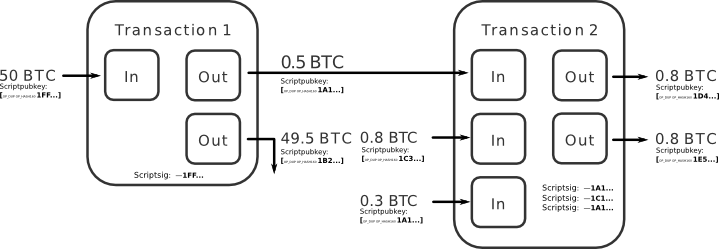
\includegraphics[width=0.6\textwidth]{utxo}
  \caption[UTXO-model]{Voorbeeld van het UTXO-model zoals in gebruik bij Bitcoin, bron: http://news.8btc.com/thoughts-on-bytom-design-extension-of-utxo-structure.}
  \label{utxo_model}
\end{wrapfigure}

Transacties bestaan uit een input en output. In plaats van het aggregeren van een balans voor elk \gls{account}, wordt er bijgehouden wat de output van een transactie is. De balans is hierbij de som van alle openstaande outputs van het desbetreffend \gls{account}. In fig. \ref{utxo_model} is te zien hoe dit in zijn werk gaat. Een onderdeel van de services die de \glspl{node} binnen het netwerk aanbieden is het valideren van transacties. Hierbij worden drie onderdelen gevalideerd:

\begin{itemize}

  \item Een output mag maar één keer geclaimd zijn.
  \item Nieuwe outputs worden alleen gecreëerd door een transactie.
  \item De som van alle waardes van de geclaimde outputs moet groter zijn als de totale som van de nieuwe gecreëerde outputs.
\end{itemize}

Wanneer dit het geval is wordt de transactie geaccepteerd en opgenomen in de lokale replica van de blockchain. Over tijd kan het voorkomen dat de replica van verschillende \glspl{node} inconsistent worden, waarbij het kan voorkomen dat er twee of meer transacties dezelfde coin meerdere malen uitgeeft. Dit staat bekend als \gls{double_spending} \citep{6688704}.

\clearpage
Een nieuw block wordt gecreëerd door het uitvoeren van het mining proces. Dit wordt uitgevoerd door zogenaamde \glspl{miner} node. Om te bepalen welke \gls{node} verantwoordelijk is voor het volgende block moet er een oplossing gevonden worden voor het proof-of-work. Dit proces zorgt ervoor dat er een beslissing gemaakt wordt over de volgorde van de transacties, en dat de inhoudt van een block niet aangepast kan worden omdat dit in directe verbinding staat met het gedane \acrshort{PoW}.

\paragraph{Discovery protocol}

Om het het netwerk te betreden worden er DNS servers benaderd waarbij gebruik wordt gemaakt van het TCP protocol. Deze DNS servers worden in stand gehouden door vrijwilligers en geven een willekeurige set aan \glspl{bootstrap_node} terug die actief zijn in het netwerk. Wanneer de \gls{node} toegetreden is tot het netwerk wordt er een \gls{peer_list} bijgehouden met alle \glspl{node} waarmee er connectie is gelegd. Deze \gls{peer_list} wordt gebruikt om connectie te leggen bij een eerstvolgende toetreding tot het netwerk.

\paragraph{Informatie propagatie}

Voor het updaten en synchroniseren van de blockchain worden er \acrfull{tx} en block berichten verstuurd. Om tegen te gaan dat \acrshort{tx}- en block berichten verstuurd worden naar \glspl{node} die al afweten van deze informatie, wordt er een \textit{inv} bericht verstuurd wanneer een transactie of een block volledig geverifieerd is. Het \textit{inv} bericht bevat een lijst van transactie- en block hashes die reeds ontvangen zijn door de verstuurder en die beschikbaar zijn om opgehaald te worden. 
\begin{wrapfigure}{r}{0.5\textwidth}
  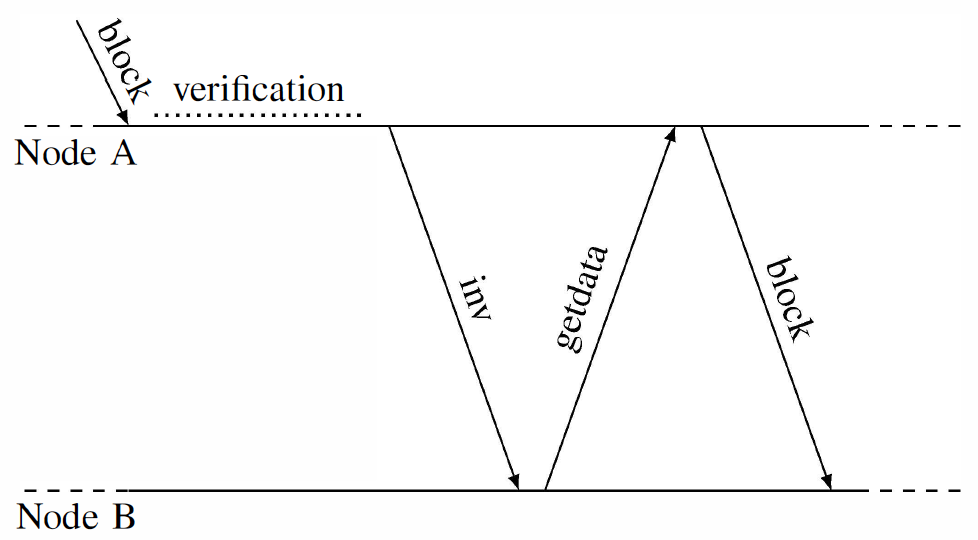
\includegraphics[width=0.5\textwidth]{bitcoin_information_propagation_0}
  \caption[Communicatie tussen deelnemers in Bitcoin]{Berichten die verzonden worden om informatie over een block uit te wisselen \citep[p.~4]{6688704}.}
  \label{bitcoin_information_propagation_0}
\end{wrapfigure}

Wanneer een \gls{node} deze informatie wilt ontvangen (bijv. omdat het de informatie nog niet heeft), wordt er een \textit{getdata} bericht verstuurd naar de verstuurder van het \textit{inv} bericht, met daarin de hashes van de informatie die de \gls{node} wilt hebben. Fig. \ref{bitcoin_information_propagation_0} visualiseert dit proces.